%%%%%%%%%%%%%%%%%%%%%%%%%%%
\chapter {Multi-Hop Location-Privacy Protection}
\label{C_MHLPP}
%%%%%%%%%%%%%%%%%%%%%%%%%%%

\section{ System Model}

\noindent Our network architecture consists of two main entities: Users and LBS Providers (LBSPs). Due to the introduction of the social network, the users' social information can be used in obfuscation forwarding process. Based on available information in the social network, the relationship between two users can be considered as friends or strangers. The user who makes a query to an LBSP will be called the original requester while the others are called intermediate users. LBSPs are located in fixed locations and their coordinates are known by all users when users join the network. Attackers are assumed to be able to access LBSPs, and attempt to locate original requesters. We assume that the LBSPs are semi-trusted and the strangers are un-trusted. We also assume that both entities have sufficient resources, like computational capability, storage and battery power.

Since two friends could be a pair of multi-hop neighbors, users can leverage Optimized Link State Routing Protocol [29] to seek friends continuously after entering the network, so that they can recognize each other and make contact in time. When a user carries an obfuscation phase query, he might send the query to a multi-hop friend through several strangers. In this case, a secure communication is necessary for between them, so that they must send the query encrypted to prevent strangers from learning anything about the query. Each user obtains a pair of asymmetric keys (public and secret key) before he joins the network from a certificate authority using well-regarded techniques, like in [28]. Whenever a user detects a new friend, he sends a request to the friend asking for his public key. In this way, a user can get his friends' public key when they encounter each other. Even though several strangers can be active in the obfuscation phase, the queries can still be securely sent to the user's friend.

The relationship strength is often ``a hidden effect of nodal profile similarities'' [30]. Let ${SV}_{i,j}$ denote a value of relationship strength which user $i$ determines whether user $j$ is an acceptable friend based on the relationship strength. For every pair of users ($i$ and $j$), we assume that there is an ${SV}_{i,j}$. If ${SV}_{i,j}$ is bigger than a specific friend threshold $T_{min}$, set by the original requester, user $j$ is considered as a friend of user $i$; otherwise, it will be treated as a stranger. The notations used in this paper and their meanings are shown in Table 3.1. 


\begin{table}
\label{table:MhlppSymbols}
\caption{MHLPP Symbols}
\centering
\begin{tabular}{|p{1.2in}|p{3.7in}|} \hline 
Parameter & Meanings \\ \hline 
\textit{N${}_{0}$} & the original requester \\ \hline 
\textit{N${}_{i}$} & if $i>0$, it denotes the friend chosen by ${N}_{i-1}$. \newline If $i=0$, it is ${N}_{0}$. \\ \hline 
\textit{N${}_{f}$} & the last friend who handles the obfuscation query \\ \hline 
\textit{N${}_{d}$} & the destination or the LBSP \\ \hline 
\textit{K${}_{i}$} & the public key of $N_i$ \\ \hline 
\textit{S${}_{i}$} & the secret key of $N_i$  \\ \hline 
\textit{q} & a query of $N_0$ \\ \hline 
\textit{r${}_{q}$} & the requirement for the query $q$ \\ \hline 
\textit{msg} & a message contains $q$ and ${r}_{q}$ \\ \hline 
\textit{Emsg${}_{i}$} & the encrypted $msg$ using ${K}_{i}$ \\ \hline 
\textit{S${}_{id}$} & the original requester's identity \\ \hline 
\textit{D${}_{id}$} & the destination's identity \\ \hline 
\textit{L${}_{s}$} & the location of ${N}_{0}$ when it sends the query to ${N}_{1}$ \\ \hline 
\textit{R${}_{p}$} & the inner radius of the obfuscation area \\ \hline 
\textit{R${}_{s}$} & the external radius of the obfuscation area  \\ \hline 
\textit{T${}_{min}$} & the social value bound for friends \\ \hline 
\textit{C${}_{max}$} & the extra path limit in each obfuscation forward \\ \hline 
\end{tabular}
\end{table}


\section{ Details of MHLPP}

\noindent MHLPP aims to protect the original requester's ($N_0$'s) location-privacy using an obfuscation path. In other words, a query $q$ which needs to be obfuscated must go through a series of friends after it leaves $N_0$. The whole process includes two parts: the obfuscation phase and the free phase. In the former phase, $q$ is only transmitted among friends, until it is sent to an area called ``$obfuscation area$''. At the end of that phase the last friend $N_f$ replaces all $N_0$'s information by its own and forwards $q$ with an arbitrary DTN forwarding protocol, like the one suggested in [31]. In this case, what attackers can learn from the database in LBSP is $N_f$'s information, so they can hardly infer the original requester's identity and location based on that information. The free phase starts when the query $q$ is forwarded by $N_f$ and ends when it reaches the LBSP. 

Because $N_f$ is the only identity the LBSP knows, the LBSP has no choice other than replying to the last friend $N_f$ when it receives the obfuscated query. The reply can be delivered with an arbitrary DTN routing protocol as the free phase query does. The friend $N_f$ should remember who is the real destination ($N_0$) of this reply, then he transmits it to $N_0$. In this way, $N_0$ is able to send a query $q$ to an LBSP while not exposing his own information.

The obfuscation phase of a query $q$ starts when the query leaves the original requester $N_0$. When a user is holding an obfuscation phase query, he starts sensing connected friends continuously, which enables it to communicate with one-hop or multi-hop neighbor friends. Even though users in the mobile network use OLSR protocol [29] to detect others automatically, they do not communicate with their friend unless they have a requirement to send an obfuscation query. Also, they do not ask their friends for public keys. Therefore, carrying an obfuscation phase query requires a user to execute MHLPP algorithm.

When $N_0$ finds the first available friend $N_1$, he asks $N_1$ for a public key $K_1$, which will enable him to encrypt his query using $K_1$. That prevent others, e.g. strangers, from learning information in the message $msg$ that that contains both $q$ and $r_q$. $r_q$ is $N_0$'s requirement for $q$, which is always sent with the query $q$ and remains constant until the end of the obfuscation phase (we discuss this in part C). Friends who get the query can infer $q$'s obfuscation area based on parameters $R_p$, $R_s$ and $L_s$ in $r_q$, which is a ring with inner radius $R_p$, external radius $R_s$ and center $L_s$. Before $N_0$ sends the query $q$ to his friend, he initializes parameter $L_s$ to his current location and encrypts $msg$ using $K_1$ to get ${Emsg}_1$ which is what $N_0$ sends to ${N}_1$.

The destination of ${Emsg}_1$ is ${N}_1$, which is a plaintext in ${Emsg}_1$, so that other intermediate users (strangers) can help $N_0$ forward ${Emsg}_1$ to ${N}_1$. In this step, strangers transmit ${Emsg}_1$ using the OLSR protocol if ${N}_1$ is a multi-hop neighbor of $N_0$. Strangers learn nothing other than the identity of ${N}_1$, because both $q$ and $r_q$ are encrypted. They cannot help attackers locate $N_0$ because they do not know ${S}_{id}$ (the identity of $N_0$) and ${D}_{id}$ (the LBSP) included in $r_q$.

When ${N}_1$ receives ${Emsg}_1$, he decrypts it with its secret key ${S}_{1}$ to get $q$ and $r_q$. If $q$ is already in the obfuscation area defined in ${r}_{q}$ (i.e., it is already in the ring), the query $q$ finishes its the obfuscation phase. Then ${N}_1$ replaces all information of $N_0$ with his own. For example, the ${S}_{id}$ is replaced with ${N}_1$. If a location is necessary for the LBS, ${N}_1$ uses his own current location and records this change in his memory before initiating the free phase. A free phase query can then be forwarded to the destination (i.e. LBSP). 

If $q$ is still in the obfuscation phase (not in the ring), ${N}_1$ performs similar actions just as $N_0$ expect modifying $r_q$. Another difference is that instead of finding friend randomly, ${N}_{1}$ would seek for a friend who is nearer in the obfuscation area, and so will the following friend. 

The detailed algorithm is explained in Algorithm 3-1 where ${N}_{x}$ is a neighbor of ${N}_{i}$ who is carrying the query $q$. Function ``$DealWithQuery$'' is responsible for dealing with a query. For $N_0$, he generates the query $q$ and its requirement $r_q$. If ${N}_{i}$ receives ${Emsg}_{i}$, he decrypts it with his own secret key ${S}_{i}$. If $q$ finished its obfuscation phase at ${N}_{i}$, $q$ will be required to be forwarded in free phase immediately. Otherwise, $q$ needs to be processed in the obfuscation process. Both $q$ and $r_q$ are stored in ${N}_{i}$ until they are sent to the next friend. ${N}_{i}$ starts detecting friends continuously if and only if ${N}_{i}$ carries one or more obfuscation phase queries. 

\begin{algorithm}
\caption{The Obfuscation Phase in MHLPP}\label{AlgObfMhlpp}
\begin{algorithmic}[1]
\Procedure{DealWithQuery}{}
\If {the current user is $N_0$} 
	\State $generate\left (q,r_q\right)$ by himself
\Else 
	\If {the current user is $N_i$, $i>0$} 
		\State $\left (q,r_q\right) \gets {Decrypt}_{S_i}\left({Emsg}_i\right)$
	\EndIf
\EndIf

\If {$q$ can switch to the free phase based on $r_q$} 
	\State $SwitchFree\left(q\right)$
\Else 
	\State $msg \gets \left (q,r_q\right)$
	\State Store $msg$
	\State Start sensing friends
\EndIf
\EndProcedure

\Procedure{WhenEncounterUser}{$N_x$}
\State $q \gets$ get query from $msg$, $r_q \gets$ get requirement from $msg$
\If{$q$ timeout}
	\State remove $msg$
	\Return
\EndIf
\If{$q$ is eligible to switch into the free phase}
	\State $SwitchFree\left(q\right)$
	\Return
\EndIf
\If{${SV}_{i,x}$ is bigger than ${T}_{min}$ in $r_q$}
	\If{it is the first hop of $q$}
		\State assign the current location to $L_s$ of $r_q$
	\EndIf
	\State ${Emsg}_x \gets {Encrypt}_{S_x}\left(q,r_q\right)$
	\State forward ${Emsg}_x$ to $N_x$
	\State remove $msg$ from memory
	\State stop sensing friends
\EndIf
\EndProcedure

\Procedure{SwitchFree}{$q$}
\State ${q^*} \gets$ replace $q$'s requester-information ($N_0$) by $N_i$
\State record $\left(q,q^*\right)$
\State forward $q^*$ with DTN protocols
\EndProcedure
\end{algorithmic}
\end{algorithm}

When ${N}_{i}$ detects a new neighbor ${N}_{x}$ (one-hop or multi-hop neighbor), he follows steps in ``\textit{WhenEncounterUser}''. For an expired query, ${N}_{i}$ simply drops it. If the query $q$ is already inside its obfuscation area, ${N}_{i}$ switches it to the free phase. If $q$ stays in the obfuscation phase and ${N}_{x}$ is an available friend, ${N}_{i}$ encrypts both $q$ and $r_q$ using ${N}_{x}$'s public key ${K}_{x}$ to get an encrypted message ${Emsg}_{x}$. Then ${N}_{i}$ forwards ${Emsg}_{x}$ to ${N}_{x}$ and stops sensing friends after ${Emsg}_{x}$ departs from it.

When we mention that ${N}_{i}$ switches a query $q$ to the free phase, ${N}_{i}$ actually replaces $N_0$'s information with its own one in $q$ to get ${q}^{*}$ and records this replacement in its storage, then ${N}_{i}$ uses the Spray and Wait protocol [31] to forward ${q}^{*}$ in plaintext. That allows ${N}_{i}$ to hide $N_0$'s identity and forward a reply from LBSP to $N_0$.


\section{ Requirement parameters}

\noindent In the obfuscation phase, ${r}_{q}$ is always in $msg$ so that friends who get $msg$ can make decisions (e.g. selections of friends) based on it.

All parameters (i.e., ${S}_{id}$, ${D}_{id}$, ${R}_{p}$, ${R}_{s}$, ${L}_{s}$ ,${T}_{min}$ and ${C}_{max}$) in ${r}_{q}$ are given by ${N}_{0}$ before ${Emsg}_{1}$ leaves ${N}_{0}$. Parameters ${S}_{id}$ and ${D}_{id}$ record the identities of ${N}_{0}$ and the destination (LBSP) ${N}_{d}$, based on which last friend ${N}_{f}$ is able to send the query freely to ${D}_{id}$ (${N}_{d}$) and forward the reply to ${S}_{id}$ (${N}_{0}$).

The obfuscation area is a ring with an inner radius ${R}_{p}$ and an external radius ${R}_{s}$. As shown in Figure 3.1-a, the obfuscation area is actually the grey area ``$a$''. Obfuscation area must guarantee both the original requester's location-privacy and location awareness. In other words, the value of ${R}_{p}$ should be big enough, so that there are sufficient users in the inner circle (with a radius ${R}_{p}$). At the same time, ${R}_{s}$ should be small enough so that the LBSP can provide a service, acceptable to ${N}_{0}$. 

\begin{figure} [H]
  \centering 
  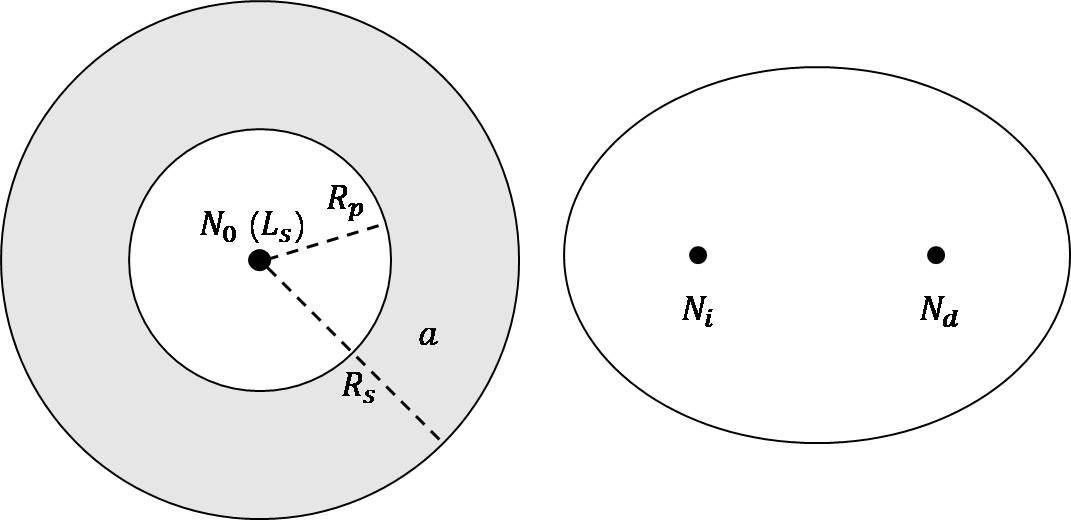
\includegraphics[width=4.0in]{figures/FIG_SelectionOfNextFriend.png}
  \caption{The selection of the next friend} 
  \label{fig:SelectionOfNxtFriend} %% label for entire figure 
\end{figure}

A user ${N}_{x}$ can be chosen by ${N}_{i}$ as a friend for $q$ if and only if ${SV}_{i,x}$ is bigger than the threshold ${T}_{min}$. The original requester ${N}_{0}$ can set various values for his queries based on their importance. If ${T}_{min}$ is large, there would be fewer friends for any users in the network which reduces the query success rate to a certain extent, as a result. We assume that the original requester can balance the level of privacy and the success ratio. 

Most DTN routing protocols aim to deliver queries through the shortest path, while MHLPP pays more attention to security in its obfuscation phase. Consequently, the obfuscation process in MHLPP results in a longer path from the original requester ${N}_{0}$ to the destination ${N}_{d}$. To limit the length of the path, we introduce parameter ${C}_{max}$ which is the maximum extra path (e.g., the difference of the length and the distance between the ${N}_{i}$ and LBSP) we can tolerate. For any friend ${N}_{i}$ who gets a ${C}_{max}$ from ${r}_{q}$, if he selects ${N}_{x}$ as the next friend, the extra path should not be longer than ${C}_{max}$. Let's denote the optimal path from user $m$ to $n$ by ${Dis}\left (m,n\right )$, and the extra path from ${N}_{i}$ to ${N}_{d}$ through ${N}_{x}$ by ${C}_{i,x,d}$. Then ${C}_{i,x,d}$ can be defined as follow.

\begin{equation} \label{GrindEQ__1_} 
C_{i,x,d} =Dis(i,x)+Dis(x,d)-Dis(i,d) 
\end{equation} 

${C}_{i,x,d}$ must be a value smaller than ${C}_{max}$. If ${Dis}\left (m,n\right )$ is the straight-line distance between point $m$ and $n$, then next friend ${N}_{x}$ should be in an ellipse ${E}_{C}$ with focus points ${N}_{i}$ and ${N}_{d}$. Let's denote the coordinate of ${N}_{i}$ by $\left(-\frac{d}{2} ,0\right)$ and the coordinate of ${N}_{d}$ by $\left(\frac{d}{2} ,0\right)$. Then, the equation of the ellipse ${E}_{C}$ is
\begin{equation} \label{GrindEQ__2_} 
\frac{x^{2} }{\left(d+C_{\max } \right)^{2} } {\rm +}\frac{y^{2} }{2d\cdot C_{\max } +C_{\max }^{2} } {\rm =}\frac{1}{4}  
\end{equation} 
As shown in Figure 3.1-a, ${L}_{s}$ is the center of the ring while ${R}_{p}$ and ${R}_{s}$ are the inner and external radii, respectively. The query $q$ switches to the free phase when it enters the ring area. 

\noindent As shown in Figure 3.1-b, ${N}_{i}$ who is carrying obfuscation queries should choose his next friend ${N}_{x}$ in the ellipse, which avoids the query $q$ going through an unacceptably long path.

\noindent In conclusion, a query $q$ starts at the center and moves inside the ring, until it reaches the obfuscation area. The point ${N}_{i}$ in Figure 3.1-b should be inside the ring, and the point ${N}_{d}$ might be anywhere. As a result, a user ${N}_{i}$ who is carrying an obfuscation query detects a friend continuously who has a larger distance from ${L}_{s}$ and inside an ellipse. If there is a friend like that, ${N}_{i}$ sends the query to that friend ${N}_{x}$.

\section{ Privacy Analysis}

\noindent We assume that attackers can achieve all information in LBSPs know. Obviously, they can know the identity of the last friend $N_f$ who replaces ${N}_{0}$'s information with his own. It is possible for the attackers to locate $N_f$ with little cost. For example, if ${N}_{0}$${}_{ }$stops moving after sending the query $q$, it is reasonable for $N_f$ to believe that ${N}_{0}$ is in a ring centered at the location of itself with radii ${R}_{p}$ and ${R}_{s}$. In other words, the distance between ${N}_{f}$ and ${N}_{0}$ should be in a range between ${R}_{p}$ and ${R}_{s}$. If attackers find all users who satisfy this condition, the original requester might be among these users with high probability. Then, a success ratio $P_{r_pr_s}$ to locate ${N}_{0}$ can be measured by a conditional probability
\begin{equation} \label{GrindEQ__3_} 
P_{r_{p} r_{s} } =p_{r_{p} r_{s} } \cdot \frac{1}{m_{r_{p} r_{s} } }  
\end{equation} 
where $P_{r_pr_s}$ is the probability that ${N}_{0}$ is in the ring (i.e., the distance between ${N}_{0}$ and ${N}_{f}$ is larger than ${R}_{p}$ and smaller than ${R}_{s}$). Here, $m_{r_pr_s}$ is the number of users who are in the ring. Attackers locate ${N}_{0}$ successfully if and only if ${N}_{0}$ is in the ring, at the same time, attackers pick the correct one from all $m_{r_pr_s}$ users at that area.

\noindent In the worst case, attackers know exact values $R_s$ and $R_p$. Then, the Eqn. \eqref{GrindEQ__3_} becomes 
\begin{equation} \label{GrindEQ__4_} 
P_{R_{p} R_{s} } =p_{_{R_{p} R_{s} } } \cdot \frac{1}{m_{_{R_{p} R_{s} } } }  
\end{equation} 
where $P_{r_pr_s}$ is the probability that ${N}_{0}$ is on the ring (i.e., the distance between ${N}_{0}$ and ${N}_{f}$ is larger than ${R}_{p}$ and smaller than ${R}_{s}$). $m_{r_pr_s}$ is the number of users who are in the ring. Since parameters (e.g., ${R}_{p}$ and ${R}_{s}$) in ${r}_{q}$ are kept secret among trusted friends in our system model, attackers can hardly get the actual values of those parameters.

\section{ Complexity discussion}

\noindent In order to guarantee secure communications among friends, encryption is introduced in our protocol. In the obfuscation phase, the query is transmitted along friends, i.e. ${N}_{0}$, ${N}_{1}$, ${N}_{2}$, ..., ${N}_{f}$. When the query is sent from ${N}_{i}$ to ${N}_{i+1}$, a pair of encryption and decryption is needed, so the number of such pairs $T_{en}$ should be equal to $f$. 

$T_{en}$ grows with both ${T}_{min}$ (threshold used to decide friend relationship) and inner radius ${R}_{p}$. Essentially, it is the number of friends participating in transmitting a query $q$ in its obfuscation phase that influences $T_{en}$. Given a smaller ${T}_{min}$, a user carrying the obfuscation phase query has more chances to encounter more friends in a certain area. A larger ${R}_{p}$ also leads to a bigger area inside the ring, so that there are more friends in this area. We evaluate the number of encryptions and decryptions in our simulation. Figure 3.2 shows the average number of encryptions ($T_{en}$) with different friend thresholds ${T}_{min}$ and inner radius ${R}_{p}$. We observe that $T_{en}$ increases steadily as we increase ${T}_{min}$ and ${R}_{p}$.

\begin{figure} [H]
  \centering 
  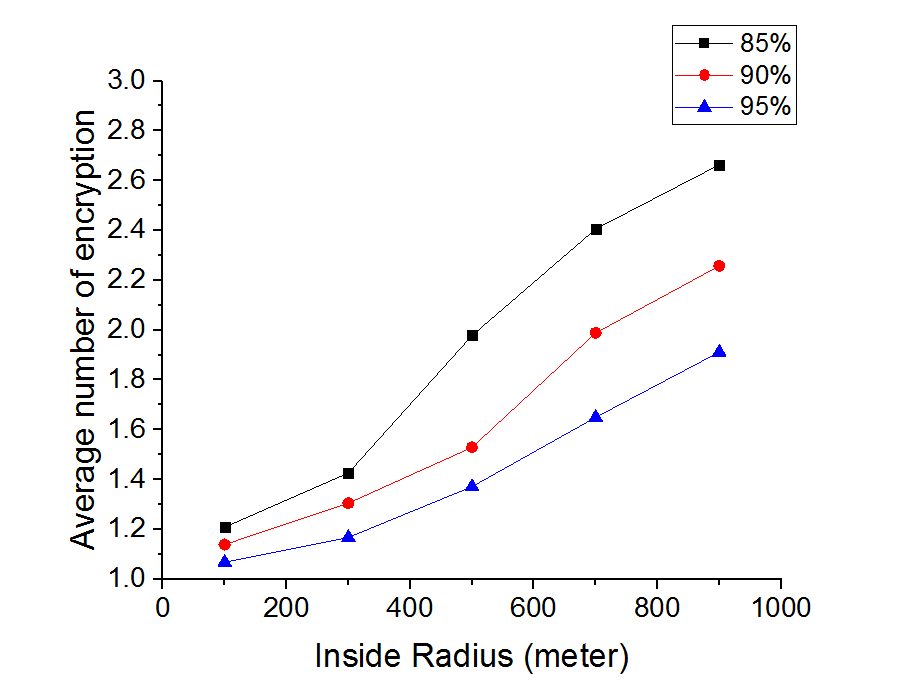
\includegraphics[width=4.0in]{figures/NumOfEncWithInnerR.png}
  \caption{The number of encryption with various inner radius} 
  \label{fig:NumOfEncWithInnerR} %% label for entire figure 
\end{figure}

It is evident that encryption and decryption process in MHLPP results in an extra cost in both energy and computational resources. However, the number of encryptions and decryptions is quite low (below 3) which reasonable based on the experiment.

\section{ Performance Analysis}

\noindent We use the map of Helsinki in our simulator to evaluate MHLPP. It is also compared against the known protocol, Hybrid and Social-aware Location-Privacy in Opportunistic mobile social networks (HSLPO). The simulation parameters are shown in Table 3.2. All pedestrians and cars are users in MHLPP. These users are moving on the map along streets continuously. There is an LBSP fixed at a random location on the map. For each user, we give him random social values between 0\% and 100\%, each corresponding to all other users. Each value has the same probability, so we can compute the expected number of friends of a user. For example, if we are given a privacy threshold (${T}_{min}$) of 85\%, then there might be 15\% (100\%-85\%) users who are friends of a certain user.

\noindent As shown in Table 3.2, there are 126 users in the map. For each of them, say user $i$, we give him 126 random $SV$ values, which denotes the relationship strength between him and other users, so that there are ${126}^2$ $SV$s in our simulation. The $SV$s are between 0 and 100. As a result, if the ${T}_{min}$ is equal to 85, the average number of friends of each user should be 18.9 (=$126\times (100-85)/100$).

\begin{table}
\label{table:MhlppExperimentParameters}
\caption{MHLPP Experiment Parameters}
\centering
\begin{tabular}{|p{2.4in}|p{3.0in}|} \hline 
Parameter & Value \\ \hline 
Simulation Time & 10 minutes \\ \hline 
Map Size (W x H) & 4500 m x 3400 m \\ \hline 
Total number of users & 126 \\ \hline 
Pedestrians/ Cars & 84/42 \\ \hline 
Communication Area Radius & 10m -- 90 m \\ \hline 
Pedestrian Speed & 1.8-5.4 Km/h \\ \hline 
Car Speed & 10-50 Km/h \\ \hline 
\end{tabular}
\end{table}

Users are placed at random locations at the beginning of each experiment. We choose another random point for each user, so that he can move back and forth along streets between that point and the point his starts at. The user speed depends on its type (pedestrians or cars) and set randomly. All queries have a 10-minute timeout. The queries which are expired before they reach the LBSP (the destination) are considered to be failed in our success ratio statistics.

\noindent Figs. 3-5 compare performances between HSLPO and MHLPP for different values of $k$, communication radius and privacy threshold (${T}_{min}$ in MHLPP). The $k$ is the privacy-level requirement in HSLPO. Both HSLPO and MHLPP have different criteria in which a query can switch to the free phase. To make them comparable, we create a new parameter, called \textit{obfuscation distance}. If a query leaves ${N}_{0}$ at location ${L}_{a}$ and switches to the free phase at ${N}_{f}$ whose location is ${L}_{b}$, then the obfuscation distance is the straight-line distance between ${L}_{a}$ and ${L}_{b}$. We test the obfuscation distances of HSLPO with different parameters, and then we set the inner radius of MHLPP to those values. The query success ratio is the ratio of delivered queries to the total number of queries. The number of hops ($h$) is the number of intermediate users between ${N}_{0}$ and the destination (LBSP). We count the number of users surrounding the last friend in a specific range, which is $k$ times the communication radius. We calculate the entropy using the reciprocal of the number of surrounding users.

\subsection{ Query success ratio}

\noindent The query success ratio is the percentage of delivered queries among a number of attempts. Based on the timeout value in Table II, a query is delivered successfully, if it arrives at the LBSP (the destination) before the timeout; otherwise it fails. We use the query success ratio to evaluate the delivery performance of MHLPP.


\noindent As shown in Figure 3.3-a, the success ratio in MHLPP is always higher than that in HSLPO. As the value of $k$ increases, HSLPO success ratio drops sharply while MHLPP remains stable. This is because the larger $k$ is, the harder it is for HSLPO to find enough friends in a limited time. The lack of friends has less impact on MHLPP. We observe that the success ratio of MHLPP rises when $k=7$. That is because it depends on the inner radius which is equal to the obfuscation distance of HSLPO. The obfuscation distance decreases when $k=7$, because most of the queries which complete their obfuscation phase have a short obfuscation distance. In Figure 3.3-b, both HSLPO and MSLPP values increase and have the same trend when given a larger communication radius. The reason is that the communication radius effects the free phase more than the obfuscation phase for both. As shown in Figure 3.3-c, higher privacy threshold leads to lower success ratio in two algorithms. Its impact on HSLPO is more intense than that on MHLPP, which is the most important characteristic of MHLPP. MHLPP has a better performance than HSLPO especially when there are fewer friends in the network. MHLPP can transmit messages with the help from strangers in its obfuscation phase while HSLPO cannot. 

\subsection{ Number of Hops}

\noindent We count the number of hops it takes for queries to be delivered successfully and calculate the average. Every user who takes part in the delivery process is considered in the hop count. We introduce this criterion to measure the routing path length of the algorithm. MHLPP is more sensitive to the probability that a user encounters a friend than HSLPO is. The reason is that MHLPP aims to reach a certain distance rather than taking certain number of hops. In other words, MHLPP continues sending queries to other friends until queries enter their obfuscation area. In this process, MHLPP takes every chance to forward queries. If it is hard for MHLPP to find friends, it can also take the queries to obfuscation areas with fewer friends. Therefore, the probability that users encounter friends has less impact on the performance of MHLPP. The result of this experiment is shown in Figure 3.4.

\noindent In Figure 3.4-a, the number of hops in HSLPO is affected by parameter $k$ obviously. Especially, the first $k$ hops forwarders must be friends, which makes it hard for HSLPO to have queries to be forwarded successfully. Both protocols have similar number of hops in their free phases, but HSLPO has exactly $k$ hops in its obfuscation phase, while MHLPP can have fewer than $k$ hops. In figure 4b, the number of hops in MHLPP grows with the communication radius obviously, while it does not change a lot in HSLPO, because only successful delivery queries are counted in the statistics. Given a large communication radius, MHLPP has a much higher success ratio for delivered queries as it can connect more friends. In Figure 3.4-c, the value of MHLPP drops for higher privacy thresholds. The reason is the same as Figure 3.4-b. For HSLPO, no matter how hard it is to find a friend, it attempts to find exactly $k$ friends. However, if it is too hard to find a friend, MHLPP's friend can carry the query while moving and complete the obfuscation process. For higher privacy thresholds (i.e. resulting in fewer friends), MHLPP chooses to carry queries other than finding friends. That results in a drop in the number of hops.


\subsection{ Security}

\noindent Since the principles with that two protocols protect original requesters are different, we evaluate the probability that attackers locate the original requester if the distance between him and the last friend is smaller than a some value $r$, which is equal to $k$ times the communication radius. Since the last friend reveals himself to the LBSP, attackers might locate him accurately. We assume that attackers know the privacy parameter $k$. In the worst case, the distance between the original requester and the last friend is smaller than $r$ when attackers start to locate the original requester. That gives attackers a chance to locate the original requester. We count all users who are inside the radius $r$ of the last friend, and the original requester is one of them. For example, if there are $m$ users in the area, the probability should be $\frac{1}{m}$. Figure 5 compares the entropy $E$ of both HSLPO and MHLPP. We use the following formula for computing entropy:
\[E=-\frac{1}{m}{log}_2\left(\frac{1}{m}\right)\] 
From Figure 3.5-a, we observe that MHLPP has very small (about 0.04) increase in entropy compared to HSLPO. When the original requester is in the circle centered at the last friend, HSLPO is a little more secure than MHLPP but not by very much. That is because HSLPO always switches to the free phase when the last friend encounters the previous friend, so the previous friend must in the circle. MHLPP does not have this condition. Both graphs in Figure 3.5-a and Figure 3.5-b have the same trend. The curve of MHLPP is also a little higher than that of HSLPO, while two curves almost meet when the communication radius is small or large. Given a small radius, the entropy of both protocols are small. When the radius is large, we can ignore the effect of the previous friend mentioned about for Figure 3.5-a as there are so many users in the circle. From Figure 3.5-c, since the circle neither expands or shrinks, we observe that the two curves exhibit similar behavior. The values of HSLPO are always lower than the correlated values of MHLPP. However, as we observed in the experiment, the last friend is always hundreds of meters away from the requester. 


